% !TeX root = ../main.tex

\chapter{评估}
\label{chap:evaluation}

为了测试模型的效果及利用模型的优化效果,本章将对使用模型进行的预测和优化进行评估。评估使用在现实环境中采集的Wi-Fi流量数据作为背景流量,在此流量上进行数据传输的模拟。Wi-Fi流量的采集在
商场(位于一座42层大楼的第3层,总面积约8000平方米),实验室
%\footnote{指在实验室房间内采集的数据,而非Wi-Fi受控的实验室环境。}
(面积200平方米)和家庭环境中(位于一座7层公寓的第3层,面积约140平方米)。数据采集的时间从上午10:30到下午9点,一共收集了长度为294小时的Wi-Fi数据。
\section{使用模型进行的预测}
本节从计算复杂度、预测的相关性、准确性和对LDPC解码效果的提升上进行评估。

\textbf{整数分解与蒙特卡罗方法的性能比较}。在第\ref{sec:model}节中,我们提到了两种用于进行预测的算法:整数分解和蒙特卡罗方法。图\ref{fig:predict_comparison}对两种算法的性能进行了比较。图\ref{fig:convergence}讨论了蒙特卡罗方法的收敛速度,横坐标代表的是模拟的次数;纵坐标是重复1000次模拟后,每次模拟结果中各个比特位置预测概率的方差的均值。可以看出,蒙特卡罗方法可以很快速的收敛,因此后续模拟中模拟的次数取为100000次。图\ref{fig:complexity}对两个算法的计算次数进行了比较。整数分解的方法在对数图随着需要预测的帧长度增加而线性增加,说明其增长是指数级别的,因此选择蒙特卡罗方法具有更高的效率。
\begin{figure}[b]
	\begin{minipage}[b]{.5\linewidth}
		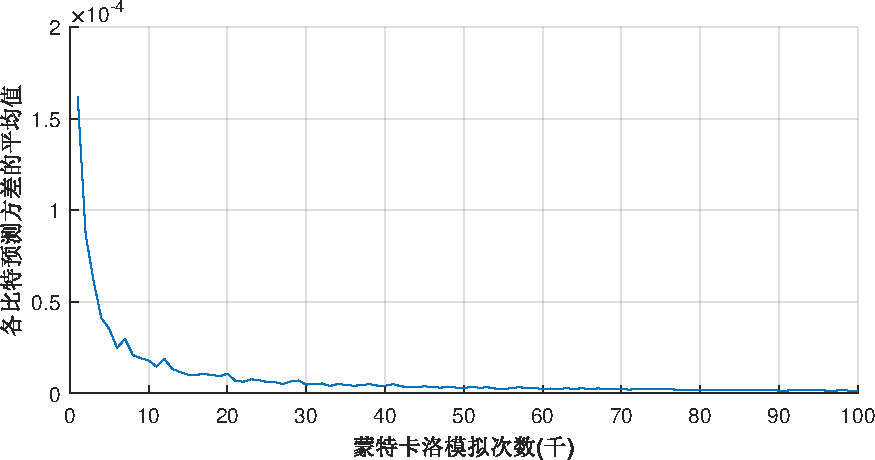
\includegraphics[width = \linewidth]{model_figure2_convergence-cropped}
		\subcaption{蒙特卡洛算法的收敛性。}\label{fig:convergence}
	\end{minipage}
	\hfill
	\begin{minipage}[b]{.5\linewidth}
		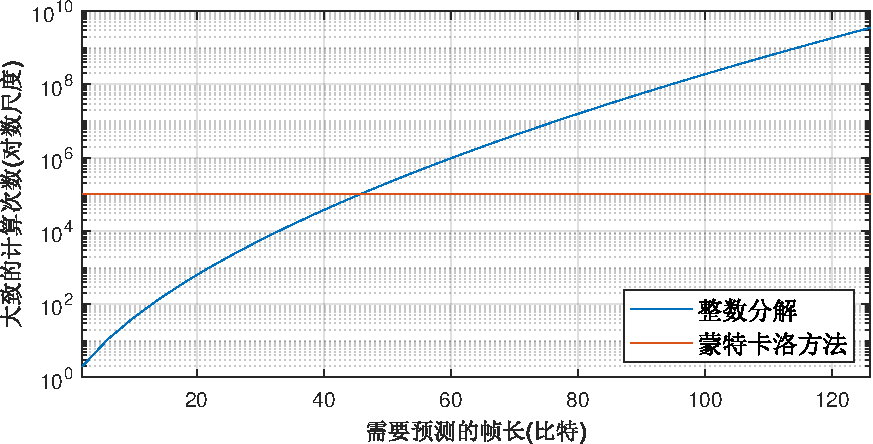
\includegraphics[width = \linewidth]{model_figure3_complexity-cropped}
		\subcaption{对数尺度下两种方法计算次数比较。}\label{fig:complexity}
	\end{minipage}
	\caption{整数分解与蒙特卡罗方法的性能比较。}\label{fig:predict_comparison}
\end{figure}

\textbf{预测的相关性}。直观上,如果两个相邻时间段的ON/OFF经验累积分布函数是相似的话,可以用前一时段的统计结果对后一时段的数据进行预测。具体实现中,给定两个时间段$\Delta_i = [t_i, t_{i+1}]$和$\Delta_{i+1} = [t_{i+1}, t_{i+2}]$。在每个时间段内,生成长度为$w$的窗口的预测,统计窗口内中ON/OFF持续时间的值。对窗口内两个时间段的ON序列和OFF序列进行柯尔莫哥洛夫-斯米尔诺夫检验(KS检验)来判断相关性。如果有$n$个窗口,假设有$0.95n$个窗口中KS检验接受了零假设,那么便可以以95\%的置信度认为两个时间段的ON/OFF分布式相似的。

图\ref{fig:kstest}对使用相邻时间段内的统计数据进行预测的可靠程度进行了分析,时间段的划分为10分钟,窗口大小为100毫秒,测试次数为1000个窗口。横轴代表测试的参数,纵轴代表KS检验的通过率,在同一横坐标下的不同点代表了不同的两个相邻时间段的通过率。在商场和家中,OFF状态存在较高的相关度,但ON状态的相关度较低;在实验室环境下,不论是ON状态还是OFF状态都存在很高的相关度,平均通过率在96.7\%和97.1\%。这说明,在中等人数且比较稳定的环境(比如实验室)下,使用该模型预测可以有比较好的效果。
\begin{figure}[t]
	\centering
	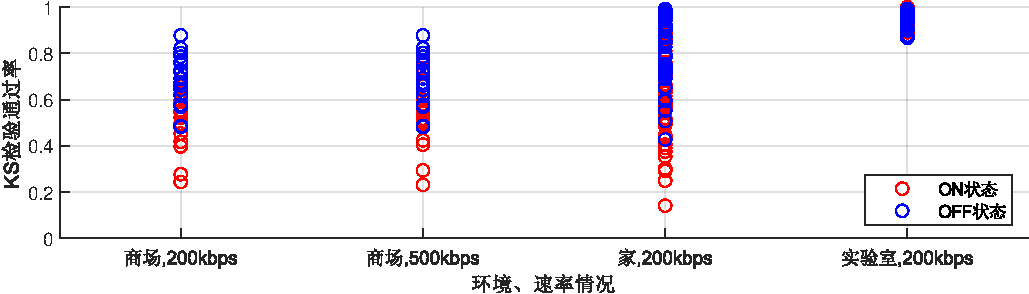
\includegraphics[width = \linewidth]{eval_figure1_sliding-cropped}
	\caption{相邻两时间窗口K-S检验的通过率。}
	\label{fig:kstest}
\end{figure}
\begin{figure}[t]
	\begin{minipage}[b]{.32\linewidth}
		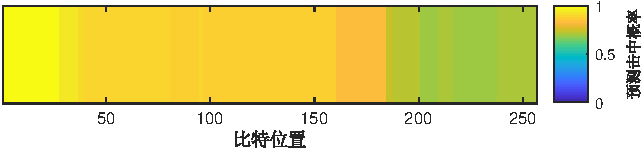
\includegraphics[width = \linewidth]{eval_figure2_1_256_500_mall-cropped}
		\subcaption{商场环境,256比特,500kbps,阈值0.6。}\label{fig:hitmap_256_500_0.6_mall}
	\end{minipage}
	\hfill
	\begin{minipage}[b]{.32\linewidth}
		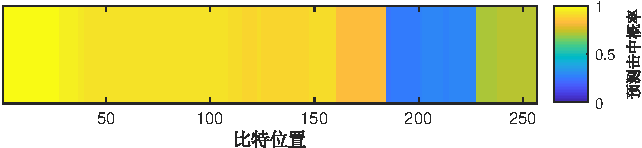
\includegraphics[width = \linewidth]{eval_figure2_2_256_500_mall-cropped}
		\subcaption{商场环境,256比特,500kbps,阈值0.5。}\label{fig:hitmap_256_500_0.5_mall}
	\end{minipage}
	\hfill
	\begin{minipage}[b]{.32\linewidth}
		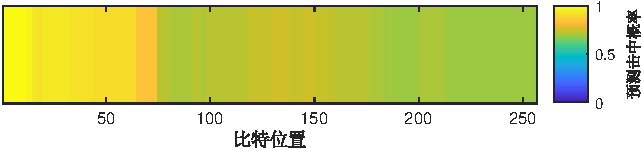
\includegraphics[width = \linewidth]{eval_figure2_1_256_200_mall-cropped}
		\subcaption{商场环境,256比特,200kbps,阈值0.6。}\label{fig:hitmap_256_200_0.6_mall}
	\end{minipage}
	
	\begin{minipage}[b]{.32\linewidth}
		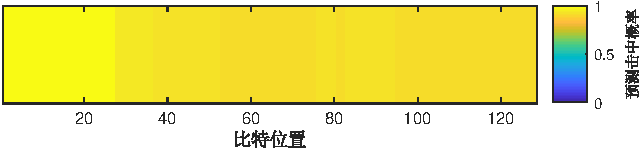
\includegraphics[width = \linewidth]{eval_figure2_1_128_500_mall-cropped}
		\subcaption{商场环境,128比特,500kbps,阈值0.6。}\label{fig:hitmap_128_500_0.6_mall}
	\end{minipage}
	\hfill
	\begin{minipage}[b]{.32\linewidth}
		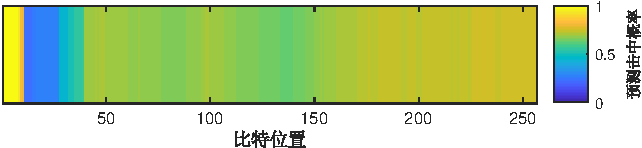
\includegraphics[width = \linewidth]{eval_figure2_1_256_500_home-cropped}
		\subcaption{家庭环境,256比特,500kbps,阈值0.6。}\label{fig:hitmap_256_500_0.6_home}
	\end{minipage}
	\hfill
	\begin{minipage}[b]{.32\linewidth}
		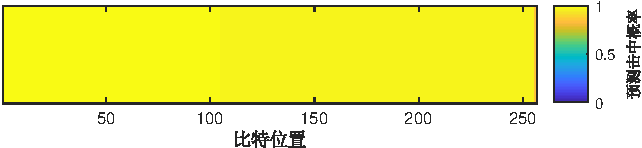
\includegraphics[width = \linewidth]{eval_figure2_1_256_500_lab-cropped}
		\subcaption{实验室环境,256比特,500kbps,阈值0.6。}\label{fig:hitmap_256_500_0.6_lab}
	\end{minipage}
	\caption{不同环境、不同帧长、不同传输速率下的预测击中热力图。}\label{fig:hitmap}
\end{figure}

\textbf{预测的准确性}。相关性在一方面评估了模型的可靠性,但受限于窗口$w$的大小并不能完整展示出模型预测的效果。一方面,过大的窗口会远离模型希望实现短时段内预测的目标;另一方面,过小的窗口不能收集足够的数据用于进行K-S检验。准确性检验了模型预测与实际发送中遇到的ON/OFF状态的符合成都。在指定阈值后(见第\ref{subsec:perm}段),概率大于阈值的部分预测为ON,不然为OFF。然后再从下一时段中随机采样到实际传输中的ON/OFF状态,将预测与真实状态进行比较,计算击中的比例,越高说明预测越准确。图\ref{fig:hitmap}展示了击中热力图,测试次数为1000次。与相关性分析比较相近的是,实验室环境的预测很准确,图\ref{fig:hitmap_256_500_0.6_lab}中平均集中率达到了98.6\%;但商场和家庭环境的预测集中率稍低,图\subref{fig:hitmap_256_500_0.6_mall}和\ref{fig:hitmap_256_500_0.6_home}的平均集中率在84.7\%和67.5\%。值得注意的是,阈值设置的比0.5稍高一些可以提升预测的效果,参照图\ref{fig:hitmap_256_500_0.6_mall}和图\ref{fig:hitmap_256_500_0.5_mall}。


\textbf{预测对LDPC解码效果的提升}。在结合预测情况下可以实施LDPC解码。图\ref{fig:ldpc}展示了在商场环境下不同帧长、不同传输速率的LDPC比特错误率。使用的是为$(96,48)$,列权重为$3$的规则LDPC码\footnote{校验矩阵来自http://www.inference.org.uk/mackay/CodesFiles.html}。可以看到,结合信道情况的解码比无信道情况的急嘛有显著的提升,图\ref{fig:ldpc_256_200}中,在SNR=14dB的情况下,预测的LDPC使得BER下降了99.8\%。蓝线是完全知道ON/OFF的具体位置情况下的LDPC解码效果。尽管使用预测信息的解码表现有一定差距,但是整体上还是比较接近的。
\begin{figure}[t]
	\begin{minipage}[b]{.32\linewidth}
		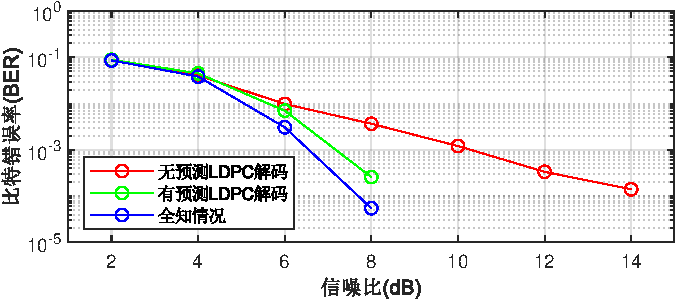
\includegraphics[width = \linewidth]{eval_figure3_LDPC_128_500_mall-cropped}
		\subcaption{商场环境,128比特,500kbps。}\label{fig:ldpc_128_500}
	\end{minipage}
	\hfill
	\begin{minipage}[b]{.32\linewidth}
		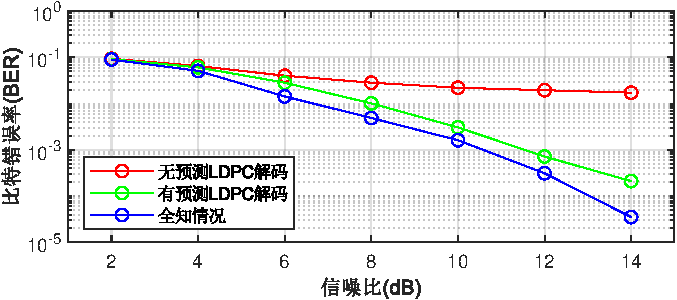
\includegraphics[width = \linewidth]{eval_figure3_LDPC_256_200_mall-cropped}
		\subcaption{商场环境,256比特,200kbps。}\label{fig:ldpc_256_200}
	\end{minipage}
	\hfill
	\begin{minipage}[b]{.32\linewidth}
		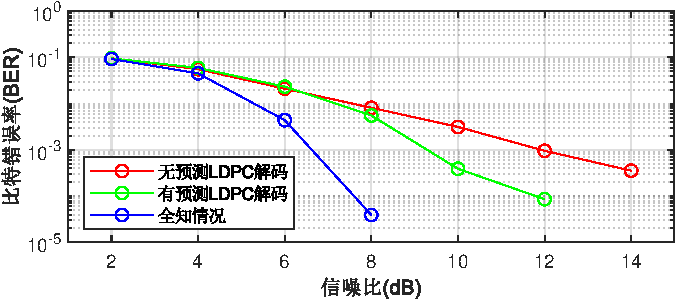
\includegraphics[width = \linewidth]{eval_figure3_LDPC_256_500_mall-cropped}
		\subcaption{商场环境,256比特,500kbps。}\label{fig:ldpc_256_500}
	\end{minipage}
	\caption{预测对LDPC解码效果的提升。}\label{fig:ldpc}
\end{figure}

\begin{figure}[t]
	\begin{minipage}[b]{.32\linewidth}
		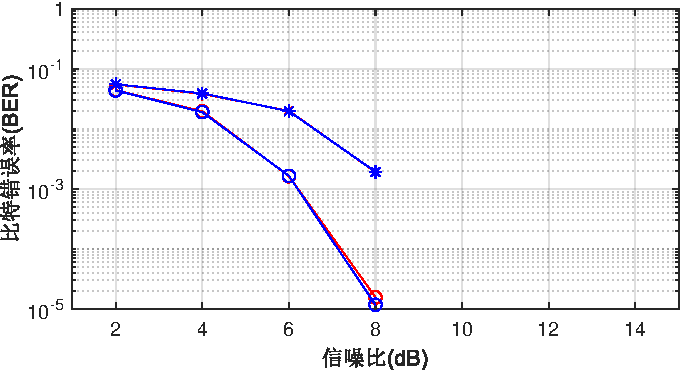
\includegraphics[width = \linewidth]{eval_figure4_allTogethrt_256_200_lab-cropped}
		\subcaption{实验室下,200kbps。}\label{fig:ber_200_lab}
	\end{minipage}
	\hfill
	\begin{minipage}[b]{.32\linewidth}
		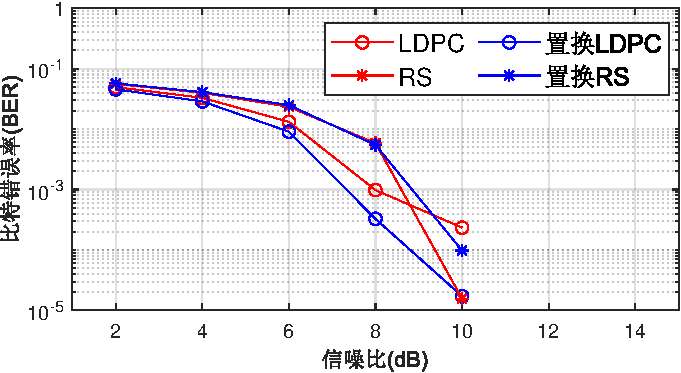
\includegraphics[width = \linewidth]{eval_figure4_allTogethrt_256_200_mall-cropped}
		\subcaption{商场下,200kbps。}\label{fig:ber_200_mall}
	\end{minipage}
	\hfill
	\begin{minipage}[b]{.32\linewidth}
		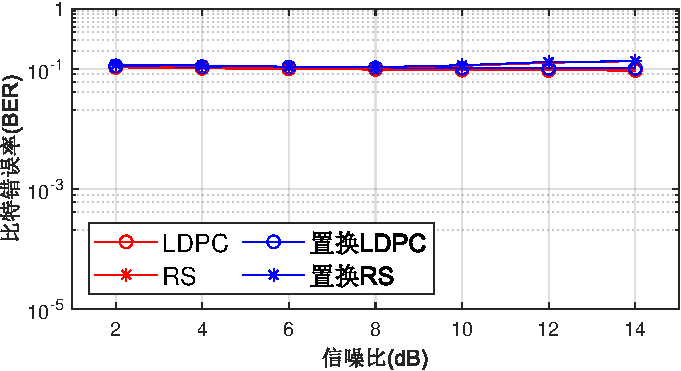
\includegraphics[width = \linewidth]{eval_figure4_allTogethrt_256_200_home-cropped}
		\subcaption{家庭下,200kbps。}\label{fig:ber_200_home}
	\end{minipage}
	
	\begin{minipage}[b]{.32\linewidth}
		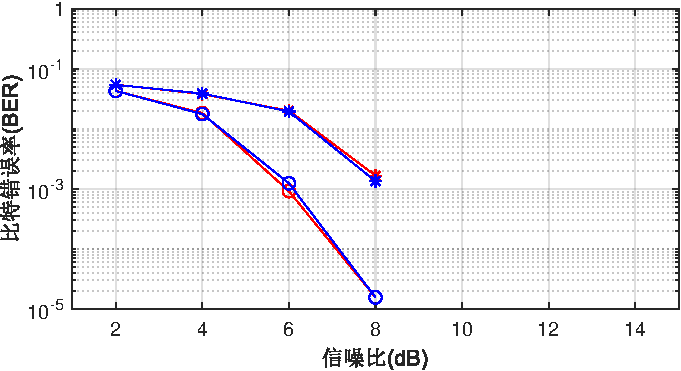
\includegraphics[width = \linewidth]{eval_figure4_allTogethrt_256_500_lab-cropped}
		\subcaption{实验室下,500kbps。}\label{fig:ber_500_lab}
	\end{minipage}
	\hfill
	\begin{minipage}[b]{.32\linewidth}
		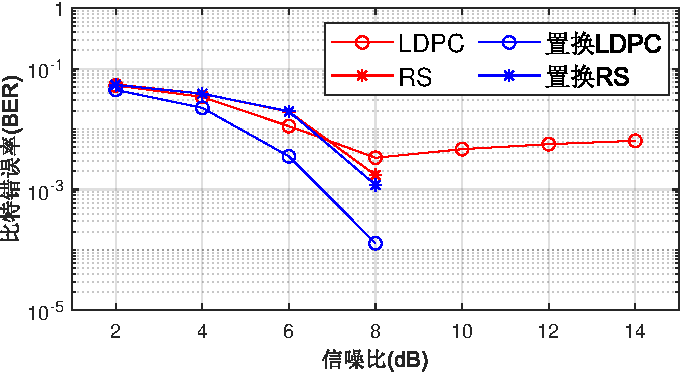
\includegraphics[width = \linewidth]{eval_figure4_allTogethrt_256_500_mall-cropped}
		\subcaption{商场下,500kbps。}\label{fig:ber_500_mall}
	\end{minipage}
	\hfill
	\begin{minipage}[b]{.32\linewidth}
		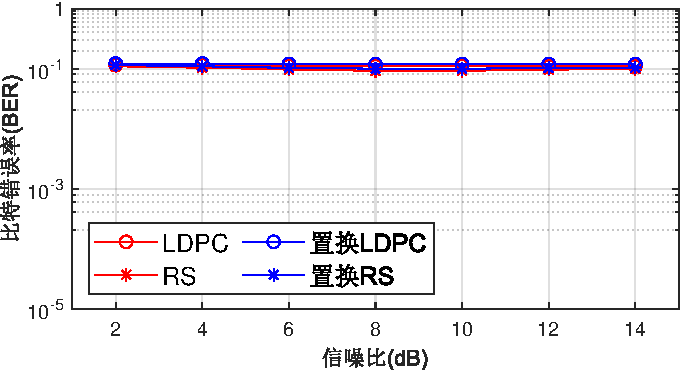
\includegraphics[width = \linewidth]{eval_figure4_allTogethrt_256_500_home-cropped}
		\subcaption{家庭下,500kbps。}\label{fig:ber_500_home}
	\end{minipage}
	
	\begin{minipage}[b]{.32\linewidth}
		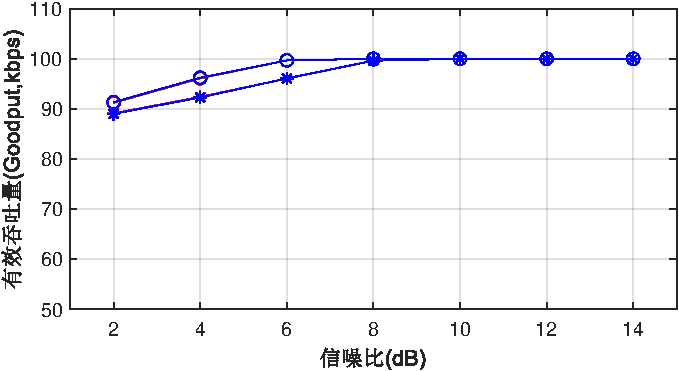
\includegraphics[width = \linewidth]{eval_figure4_goodput_256_200_lab-cropped}
		\subcaption{实验室下,200kbps。}\label{fig:goodput_200_lab}
	\end{minipage}
	\hfill
	\begin{minipage}[b]{.32\linewidth}
		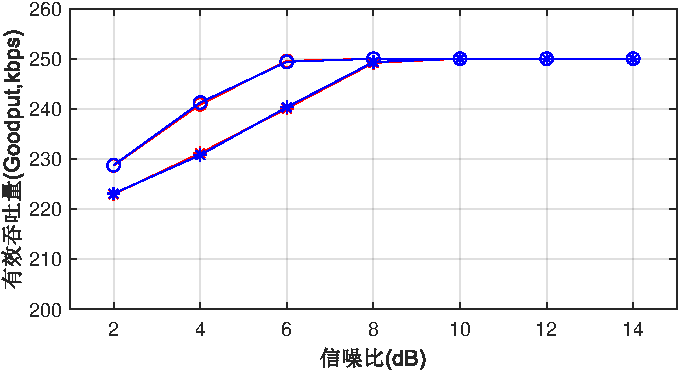
\includegraphics[width = \linewidth]{eval_figure4_goodput_256_500_lab-cropped}
		\subcaption{实验室下,500kbps。}\label{fig:goodput_500_lab}
	\end{minipage}
	\hfill
	\begin{minipage}[b]{.32\linewidth}
		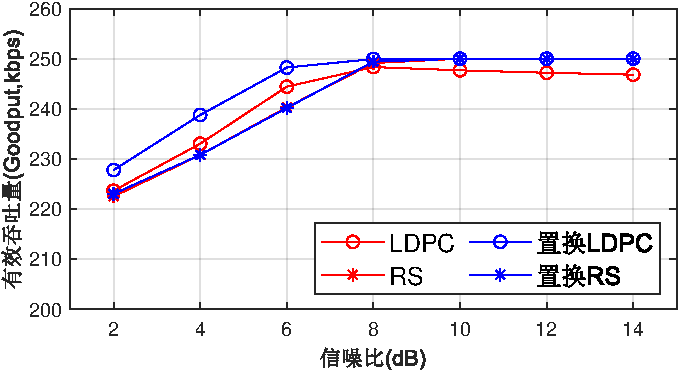
\includegraphics[width = \linewidth]{eval_figure4_goodput_256_500_mall-cropped}
		\subcaption{商场下,500kbps。}\label{fig:goodput_500_mall}
	\end{minipage}
	
	\caption{LDPC、置换LDPC、RS、置换RS比特错误率和有效吞吐量比较(帧长为256比特)。}\label{fig:ber}
\end{figure}
\section{使用模型进行的优化}

\textbf{置换对LDPC和RS码的性能提升}。图\ref{fig:ber}展示了在三种环境下,使用不同速率和编码方式的比特错误率和有效传输率表现。其中,使用的是为$(96,48)$,列权重为$3$的规则LDPC码;RS为$(31,15)$的编码,有效传输率由单位时间内被正确传输的信息计算。
实验室环境下,两种编码方式表现稳定,采用不同速率也表现稳定,这与之前对实验室的预测ON状态持续保持在近95\%以上时间保持一致。而商场中,由于存在更多的OFF状态,LDPC的表现比实验室下要差一些,但RS的表现比较稳定,这与RS本身的适合解码突发错误的特性有关;家庭下,由于OFF状态太长,导致突发错误过多,超出了两种编码的恢复能力,因此比特错误率稳定呈直线。

总体来看,LDPC的表现优于RS,但这是在牺牲运算速度的情况下;通常RS编码由专用的加速硬件。同时,能看出置换可以对系统表现进行一定的提升,在商场环境下LDPC比特错误率的下降。但对于RS码,置换的效果有限,这可能是由RS不依靠信道先验概率影响,只考虑错误发生的位置,使得置换前后影响的码元数没有大的变化;而LDPC在置换后原有不受影响的块受到了OFF状态的影响,且受先验概率的不准确导致这些不受影响的块在使用信念传播算法的过程中错误率提升,导致最终总体看来比特错误有下降。

在有效吞吐率方面,在低信噪比的情况下几乎都可以有效的传输数据,而在较高信噪比下与各个编码在对应环境下的比特错误率表现也是一致的。相差最大的情况下(实验室,500kbps,SNR=4dB),LDPC相比RS实现了5\%的提升(11kbps)。

\begin{figure}[t]
	\begin{minipage}[b]{.32\linewidth}
		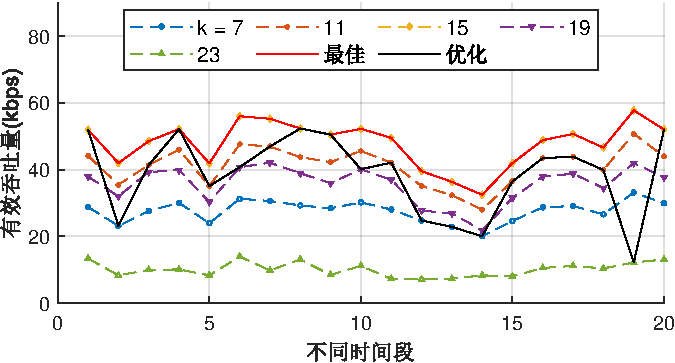
\includegraphics[width = \linewidth]{eval_figure5_optCodeRate_256_200_mall_8-cropped}
		\subcaption{商场环境,256比特,200kbps。}\label{fig:coderate_256_200_mall}
	\end{minipage}
	\hfill
	\begin{minipage}[b]{.32\linewidth}
		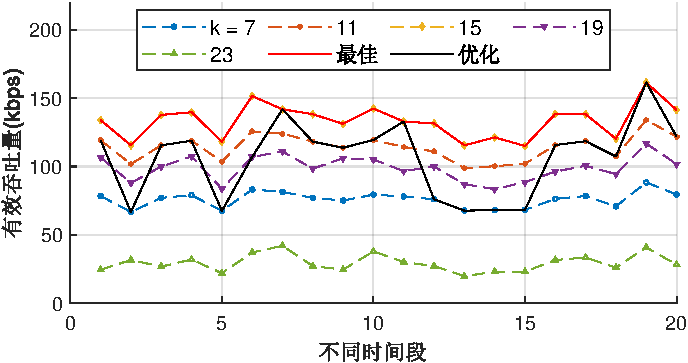
\includegraphics[width = \linewidth]{eval_figure5_optCodeRate_256_500_mall_8-cropped}
		\subcaption{商场环境,256比特,500kbps。}\label{fig:coderate_256_500_mall}
	\end{minipage}
	\hfill
	\begin{minipage}[b]{.32\linewidth}
		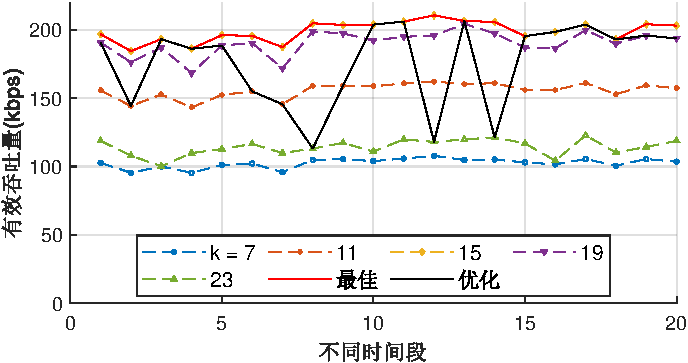
\includegraphics[width = \linewidth]{eval_figure5_optCodeRate_128_500_mall_8-cropped}
		\subcaption{商场环境,128比特,500kbps。}\label{fig:coderate_128_500_mall}
	\end{minipage}

	\begin{minipage}[b]{.32\linewidth}
		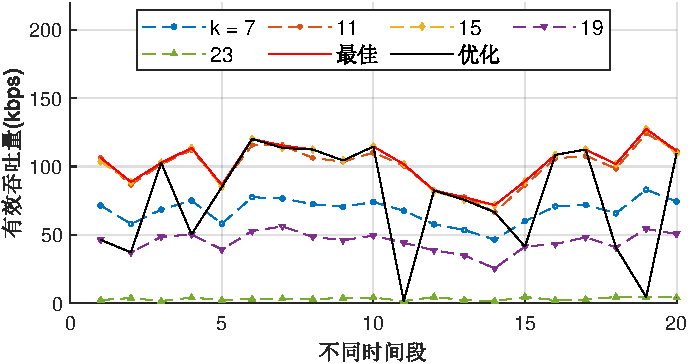
\includegraphics[width = \linewidth]{eval_figure5_optCodeRate_512_500_mall_8-cropped}
		\subcaption{商场环境,512比特,500kbps。}\label{fig:coderate_512_500_mall}
	\end{minipage}
	\hfill
	\begin{minipage}[b]{.32\linewidth}
		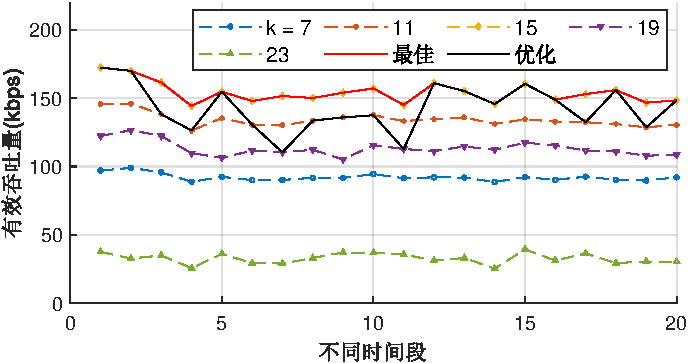
\includegraphics[width = \linewidth]{eval_figure5_optCodeRate_256_500_lab_8-cropped}
		\subcaption{实验室环境,256比特,500kbps。}\label{fig:coderate_256_200_lab}
	\end{minipage}
	\hfill
	\begin{minipage}[b]{.32\linewidth}
		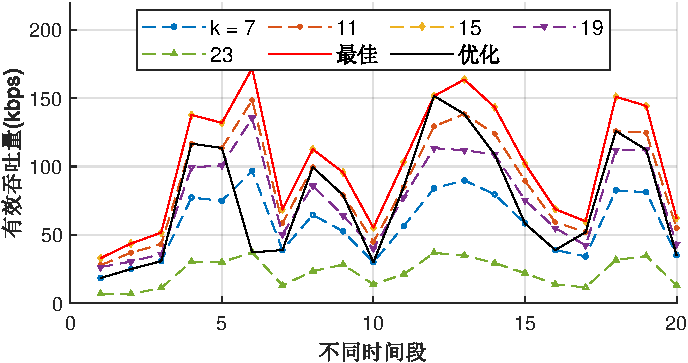
\includegraphics[width = \linewidth]{eval_figure5_optCodeRate_256_500_home_8-cropped}
		\subcaption{家庭环境,256比特,500kbps。}\label{fig:coderate_256_200_home}
	\end{minipage}
	\caption{不同环境下动态调节码率对实际吞吐量的影响。}\label{fig:coderate}
\end{figure}
\textbf{对RS码的动态参数调节}。
图\ref{fig:coderate}展示了在不同环境、速率和帧长下,利用模型的预测结果对里德-所罗门码码率调节的效果。这里采用的时$(31, k)$的里德-所罗门码。横坐标表示不同的时间段,纵坐标时实际吞吐量。在商场环境下,不同帧长和速率会有不同的ON/OFF统计特征,这也表现在图中$k$值从上到下的顺序会发生改变。图\ref{fig:coderate_256_200_mall}-\subref{fig:coderate_128_500_mall}中,在$k = 15$都达到了最高的有效吞吐量,在错误恢复和传输信息之间取得了平衡。从结果来看,预测的效果能够以平均65\%的概率击中最好的两个码率;在没有选择最佳两个码率的情况下,多数选择了高码率的情况。这可能来源于对长度的平衡不够合理。总体来看,在商场环境下使用预测优化的码率能够达到最佳吞吐量的80.79\%,最好的情况下达到88.25\%。

对比商场、实验室和家庭三种环境下的有效吞吐量,我们可以发现:1)基于预测选择的码率的最优两个码率的击中率与ON/OFF状态预测的击中率正相关。实验室环境下状态预测更准确,因此最优两个码率的击中率能达到80\%,高于商场的65\%;而家庭环境中状态预测不够准确,因此最优两个码率的击中率仅为45\%。2)基于预测选择的码率随着环境中ON/OFF统计特征的变化而变化。这在图\ref{fig:coderate_256_200_home}中表现最为明显:家庭下的ON/OFF状态变化比较剧烈,最优码率呈现上下起伏的变化,而预测给出的码率(图中黑线)也伴随着这种趋势选择不同的码率。3)在实验室条件下,使用预测优化的码率能够达到最佳吞吐量的89.63\%;而在家庭下能达到65.85\%。

